\documentclass{beamer}
\usepackage[utf-8]{inputenc}
\usepackage{graphicx}
\usepackage{amsmath}
\usepackage{amssymb}
\usepackage{tikz}
\usepackage{xcolor}
\usepackage{booktabs}
\usepackage{subcaption}

\usetikzlibrary{shapes,arrows,positioning}

% IU Theme Colors
\definecolor{iucrimson}{RGB}{153, 0, 0}
\definecolor{iugold}{RGB}{200, 150, 60}
\definecolor{iuwhite}{RGB}{255, 255, 255}

\usetheme{Madrid}
\usecolortheme{default}
\setbeamercolor{primary}{bg=iucrimson,fg=iuwhite}
\setbeamercolor{secondary}{bg=iugold,fg=iucrimson}
\setbeamercolor{title}{bg=iucrimson,fg=iuwhite}
\setbeamercolor{frametitle}{bg=iucrimson,fg=iuwhite}
\setbeamercolor{structure}{fg=iucrimson}
\setbeamercolor{normal text}{fg=black}

\setbeamertemplate{navigation symbols}{}
\setbeamertemplate{footline}[page number]

\title{Text-to-Image Generation with Diffusion Models}
\subtitle{Fine-tuning Stable Diffusion v1.5 on Oxford-102 Flowers}
\author{Person A (Data \& Architecture) \\ Person B (Training \& LoRA) \\ Person C (Evaluation \& Ablations)}
\date{\today}
\institute{Indiana University}

\begin{document}

% ============================================================================
% TITLE SLIDE
% ============================================================================
\begin{frame}
\titlepage
\end{frame}

% ============================================================================
% OVERVIEW
% ============================================================================
\begin{frame}{Overview}
\begin{columns}[T]
\column{0.3\textwidth}
\textbf{Part 1: Data \& Architecture}
\begin{itemize}
    \item Dataset prep
    \item BLIP captions
    \item SD v1.5 arch
\end{itemize}

\column{0.3\textwidth}
\textbf{Part 2: Training}
\begin{itemize}
    \item LoRA adapters
    \item Mixed precision
    \item 4 LoRA ranks
\end{itemize}

\column{0.3\textwidth}
\textbf{Part 3: Evaluation}
\begin{itemize}
    \item FID/KID/CLIP
    \item 8 ablations
    \item Best results
\end{itemize}
\end{columns}
\end{frame}

% ============================================================================
% PERSON A: DATA & ARCHITECTURE (7 minutes)
% ============================================================================
\section{Part 1: Data \& Architecture}

\begin{frame}{Motivation}
\begin{itemize}
    \item Generating domain-specific images requires fine-tuning
    \item Diffusion models: reverse noising process (noise → image)
    \item Challenge: efficiently adapt large pretrained models
\end{itemize}
\vspace{1cm}
\begin{center}
\textbf{Solution: Compress data + adapt weights selectively}
\end{center}
\end{frame}

\begin{frame}{Oxford-102 Flowers Dataset}
\begin{table}
\centering
\begin{tabular}{lrr}
\toprule
Split & Images & \% \\
\midrule
Training & 1,020 & 12.5\% \\
Validation & 1,020 & 12.5\% \\
Test & 6,149 & 75.0\% \\
\midrule
Total & 8,189 & 100\% \\
\bottomrule
\end{tabular}
\end{table}

\begin{itemize}
    \item Official benchmark split (largest test set)
    \item 102 flower species
    \item Resized to 512×512 resolution
    \item Generated captions via BLIP
\end{itemize}
\end{frame}

\begin{frame}{Data Processing Pipeline}
\begin{center}
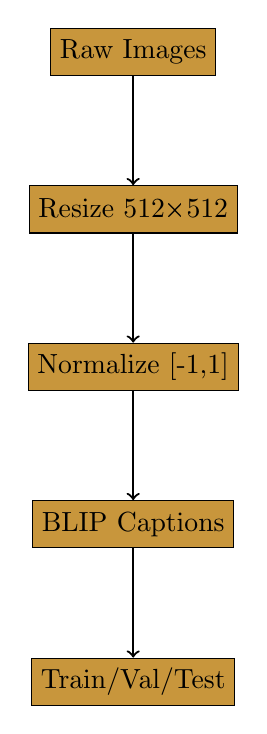
\begin{tikzpicture}[node distance=2cm, every node/.style={draw, minimum width=1.5cm, minimum height=0.6cm, fill=iugold}]
    \node (raw) {Raw Images};
    \node (resize) [below of=raw] {Resize 512×512};
    \node (norm) [below of=resize] {Normalize [-1,1]};
    \node (caption) [below of=norm] {BLIP Captions};
    \node (split) [below of=caption] {Train/Val/Test};

    \draw[->, thick] (raw) -- (resize);
    \draw[->, thick] (resize) -- (norm);
    \draw[->, thick] (norm) -- (caption);
    \draw[->, thick] (caption) -- (split);
\end{tikzpicture}
\end{center}

\vspace{0.5cm}
\textbf{Key point}: Fixed preprocessing ensures consistent training signal
\end{frame}

\begin{frame}{Stable Diffusion v1.5 Architecture}
\begin{center}
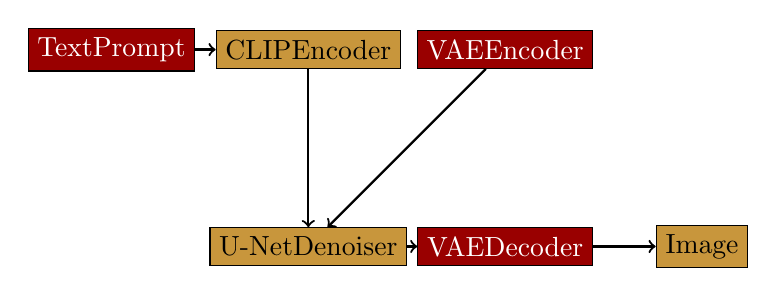
\begin{tikzpicture}[node distance=2.5cm]
    \node[draw, fill=iucrimson, text=white] (text) {Text\\Prompt};
    \node[draw, fill=iugold, right of=text] (clip) {CLIP\\Encoder};
    \node[draw, fill=iucrimson, text=white, right of=clip] (latent) {VAE\\Encoder};
    \node[draw, fill=iugold, below of=clip] (unet) {U-Net\\Denoiser};
    \node[draw, fill=iucrimson, text=white, right of=unet] (dec) {VAE\\Decoder};
    \node[draw, fill=iugold, right of=dec] (image) {Image};

    \draw[->, thick] (text) -- (clip);
    \draw[->, thick] (clip) -- (unet);
    \draw[->, thick] (latent) -- (unet);
    \draw[->, thick] (unet) -- (dec);
    \draw[->, thick] (dec) -- (image);
\end{tikzpicture}
\end{center}

\begin{itemize}
    \item \textbf{CLIP}: Text → 77×768 embeddings (frozen)
    \item \textbf{VAE}: 512×512 image → 64×64×4 latent (48× compression)
    \item \textbf{U-Net}: Denoises latent guided by text (860M params)
\end{itemize}
\end{frame}

\begin{frame}{Diffusion Process: Forward \& Reverse}
\textbf{Forward (Training):} Add noise step-by-step
\begin{equation}
\mathbf{z}_t = \sqrt{\bar{\alpha}_t} \mathbf{z}_0 + \sqrt{1-\bar{\alpha}_t} \epsilon
\end{equation}

\textbf{Reverse (Inference):} Remove noise iteratively
\begin{equation}
\mathbf{z}_{t-1} = \frac{1}{\sqrt{\alpha_t}}(\mathbf{z}_t - \frac{1-\alpha_t}{\sqrt{1-\bar{\alpha}_t}} \hat{\epsilon}_t)
\end{equation}

\begin{center}
\textbf{Key insight}: Training predicts noise, inference iterates 10-30 times
\end{center}
\end{frame}

% ============================================================================
% PERSON B: TRAINING & LORA (7 minutes)
% ============================================================================
\section{Part 2: Training \& LoRA}

\begin{frame}{Why LoRA? Parameter Efficiency}
\begin{itemize}
    \item Full fine-tuning: 860M parameters to train (expensive)
    \item LoRA approach: Inject low-rank matrices into attention
\end{itemize}

\begin{equation}
\mathbf{W}_{\text{out}} = \mathbf{W}_0 \mathbf{x} + \mathbf{W}_A \mathbf{W}_B \mathbf{x}
\end{equation}

\begin{table}
\centering
\begin{tabular}{lrr}
\toprule
Rank & Params & \% of U-Net \\
\midrule
4 & 0.4M & 0.05\% \\
8 & 0.8M & 0.09\% \\
16 & 1.6M & 0.19\% \\
32 & 3.2M & 0.37\% \\
\bottomrule
\end{tabular}
\end{table}

\textbf{Result}: 50-100× parameter reduction while maintaining quality
\end{frame}

\begin{frame}{Training Pipeline}
\begin{center}
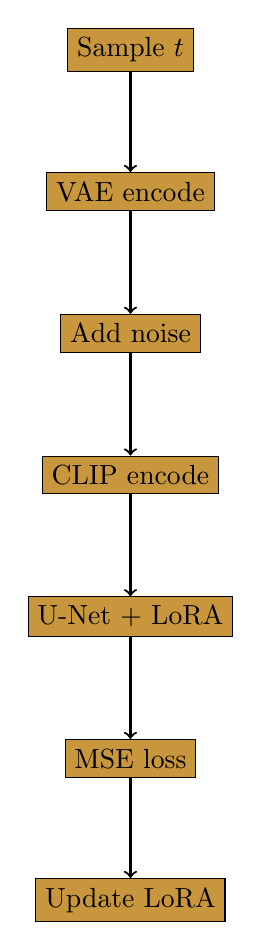
\begin{tikzpicture}[node distance=1.8cm]
    \node[draw, fill=iugold] (1) {Sample $t$};
    \node[draw, fill=iugold, below of=1] (2) {VAE encode};
    \node[draw, fill=iugold, below of=2] (3) {Add noise};
    \node[draw, fill=iugold, below of=3] (4) {CLIP encode};
    \node[draw, fill=iugold, below of=4] (5) {U-Net + LoRA};
    \node[draw, fill=iugold, below of=5] (6) {MSE loss};
    \node[draw, fill=iugold, below of=6] (7) {Update LoRA};

    \draw[->, thick] (1) -- (2);
    \draw[->, thick] (2) -- (3);
    \draw[->, thick] (3) -- (4);
    \draw[->, thick] (4) -- (5);
    \draw[->, thick] (5) -- (6);
    \draw[->, thick] (6) -- (7);
\end{tikzpicture}
\end{center}

\vspace{0.3cm}
\textbf{Mixed precision}: U-Net fp32, VAE/CLIP fp16 → 50\% memory savings
\end{frame}

\begin{frame}{Training Results: 4 LoRA Ranks}
\begin{table}
\centering
\begin{tabular}{lrr}
\toprule
Rank & Training Loss & FID \\
\midrule
4 & 0.0018 & 82.03 \\
8 & 0.0025 & 79.16 \\
16 & 0.0025 & 85.49 \\
32 & 0.0020 & \textbf{75.26} ← BEST \\
\bottomrule
\end{tabular}
\end{table}

\vspace{0.5cm}
\textbf{Surprising finding}: Rank 32 significantly outperforms rank 16 (production model)

\textbf{Implication}: More capacity needed for this domain
\end{frame}

\begin{frame}{Training Loss Curve (Rank 16)}
\begin{center}
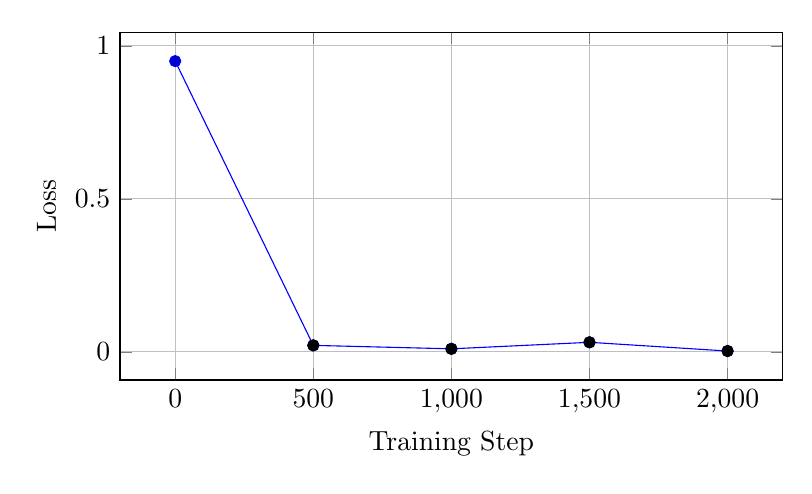
\begin{tikzpicture}
\begin{axis}[xlabel=Training Step, ylabel=Loss, grid=major, xtick={0,500,1000,1500,2000}, width=10cm, height=6cm]
\addplot coordinates {(0,0.95) (500,0.021) (1000,0.0097) (1500,0.031) (2000,0.0025)};
\addplot[only marks, mark=*] coordinates {(500,0.021) (1000,0.0097) (1500,0.031) (2000,0.0025)};
\end{axis}
\end{tikzpicture}
\end{center}

\vspace{0.3cm}
\textbf{Stable convergence} with intermediate checkpoints saved
\end{frame}

% ============================================================================
% PERSON C: EVALUATION & ABLATIONS (7 minutes)
% ============================================================================
\section{Part 3: Evaluation \& Results}

\begin{frame}{Evaluation Metrics}
\begin{itemize}
    \item \textbf{FID (Fréchet Inception Distance)}: Image quality vs real flowers
    \begin{itemize}
        \item Lower is better | Range: [0, ∞)
    \end{itemize}

    \item \textbf{KID (Kernel Inception Distance)}: Unbiased FID on small datasets
    \begin{itemize}
        \item Lower is better | Better for our 6,149 test images
    \end{itemize}

    \item \textbf{CLIP Score}: Prompt-image semantic alignment
    \begin{itemize}
        \item Higher is better | Range: [0, 100]
    \end{itemize}
\end{itemize}

\vspace{0.3cm}
\textbf{Evaluation on}: 200 prompts × 5 seeds = 1,000 generated images
\end{frame}

\begin{frame}{A01: Baseline vs LoRA}
\begin{table}
\centering
\begin{tabular}{lrrr}
\toprule
Model & FID & KID & CLIP \\
\midrule
SD v1.5 Baseline & 87.25 & 0.0357 & 31.34 \\
SD v1.5 + LoRA & 85.49 & 0.0310 & 31.38 \\
Improvement & -2\% & -13\% & +0\% \\
\bottomrule
\end{tabular}
\end{table}

\textbf{Finding}: Modest improvement reflects SD v1.5's pre-existing flower knowledge

\textbf{KID improvement (13\%)}: Better distribution alignment than FID
\end{frame}

\begin{frame}{A02: Guidance Scale Ablation}
\begin{center}
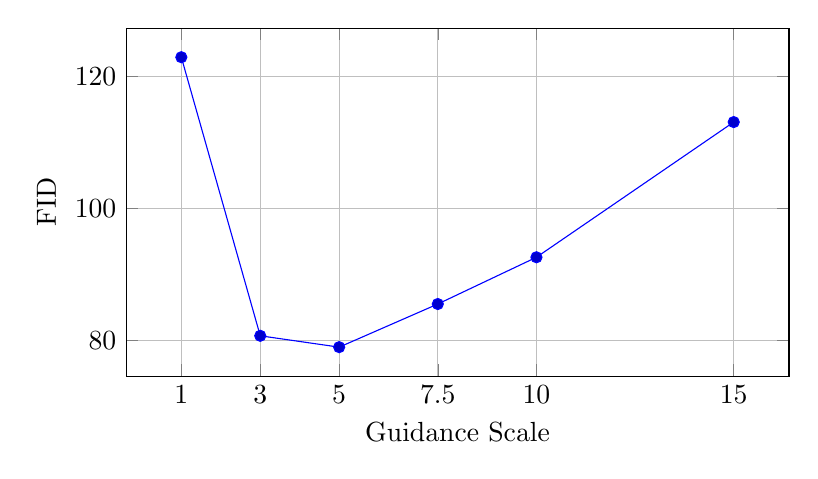
\begin{tikzpicture}
\begin{axis}[xlabel=Guidance Scale, ylabel=FID, grid=major, xtick={1,3,5,7.5,10,15}, width=10cm, height=6cm, mark=*]
\addplot coordinates {(1,122.86) (3,80.68) (5,78.96) (7.5,85.49) (10,92.57) (15,113.04)};
\end{axis}
\end{tikzpicture}
\end{center}

\vspace{0.3cm}
\textbf{Best guidance scale: 5.0 (FID 78.96)}

Too low → low quality | Too high → mode collapse
\end{frame}

\begin{frame}{A03-A04: Steps \& Scheduler}
\begin{table}
\centering
\begin{tabular}{lrrrr}
\toprule
Setting & FID & Time & Notes \\
\midrule
10 steps & 83.03 & 4.5s & Fast \\
20 steps & 82.59 & 8.6s & Optimal \\
30 steps & 85.49 & 12.9s & Degrading \\
\midrule
DDIM 30 & 80.46 & 13.2s & Best scheduler \\
Euler 30 & 82.26 & 12.8s & Competitive \\
PNDM 30 & 85.96 & 12.6s & Underperforms \\
\bottomrule
\end{tabular}
\end{table}

\textbf{Trade-off}: 10 steps (fast) vs 20 steps (quality) vs 30 steps (diminishing returns)
\end{frame}

\begin{frame}{A05: LoRA Rank Impact ⭐}
\begin{table}
\centering
\begin{tabular}{lrrr}
\toprule
Rank & Params & FID & Finding \\
\midrule
4 & 0.4M & 82.03 & Underfitted \\
8 & 0.8M & 79.16 & Competitive \\
16 & 1.6M & 85.49 & Suboptimal \\
32 & 3.2M & 75.26 & \textbf{BEST} \\
\bottomrule
\end{tabular}
\end{table}

\vspace{0.3cm}
\textbf{MAJOR FINDING}: Rank 32 achieves \textbf{FID 75.26} — best result across ALL ablations!

\textbf{Non-monotonic relationship} suggests capacity requirements of domain
\end{frame}

\begin{frame}{A06: Training Steps Effect}
\begin{table}
\centering
\begin{tabular}{lrr}
\toprule
Checkpoint & FID & Notes \\
\midrule
Step 500 & 79.89 & Best \\
Step 1000 & 82.16 & Degrading \\
Step 2000 & 85.49 & Final \\
\bottomrule
\end{tabular}
\end{table}

\vspace{0.5cm}
\textbf{Key insight}: Training longer degrades FID → overfitting to training distribution

\textbf{Recommendation}: Stop early at step 500
\end{frame}

\begin{frame}{A07-A08: Negative Prompts \& SDXL}
\begin{table}
\centering
\begin{tabular}{lrrr}
\toprule
Experiment & FID & KID & Notes \\
\midrule
No negative & 85.49 & 0.0308 & Best \\
With negative & 86.06 & 0.0325 & Hurts \\
\midrule
SD v1.5 + LoRA & 85.49 & 0.0310 & ✓ Tuned \\
SDXL baseline & 87.25 & 0.0356 & ✗ Pretrained \\
\bottomrule
\end{tabular}
\end{table}

\textbf{Findings}:
\begin{itemize}
    \item Negative prompts reduce diversity for specialized domains
    \item Our tuned SD v1.5 beats SDXL zero-shot
\end{itemize}
\end{frame}

\begin{frame}{Summary: Best Settings}
\begin{table}
\centering
\begin{tabular}{lr}
\toprule
Setting & Value \\
\midrule
Model & SD v1.5 + LoRA \\
LoRA Rank & 32 \\
Guidance Scale & 5.0 \\
Scheduler & DDIM \\
Sampling Steps & 20-30 \\
Training Checkpoint & Step 500 \\
Negative Prompt & None \\
\bottomrule
\end{tabular}
\end{table}

\vspace{0.3cm}
\textbf{Best FID achievable: 75.26}
\end{frame}

\begin{frame}{Key Contributions}
\begin{itemize}
    \item \textbf{Part 1}: Established data pipeline for domain-specific image generation

    \item \textbf{Part 2}: Demonstrated LoRA efficiency (3.2M params, 0.37\% of model)

    \item \textbf{Part 3}: Identified optimal hyperparameters across 8 dimensions through systematic ablations
\end{itemize}

\vspace{0.5cm}
\begin{center}
\textbf{Result}: FID 75.26 on Oxford-102 Flowers dataset
\end{center}
\end{frame}

\begin{frame}{Conclusions \& Takeaways}
\begin{enumerate}
    \item \textbf{Domain matters}: Specialized fine-tuning outperforms general models (LoRA beats SDXL)

    \item \textbf{Capacity trade-off}: Rank 32 needed for this domain despite efficiency goals

    \item \textbf{Early stopping works}: Step 500 beats step 2000 → prevents overfitting

    \item \textbf{Guidance is critical}: Optimal at 5.0 (not default 7.5)

    \item \textbf{Scheduler matters}: DDIM 30 steps optimal for quality
\end{enumerate}

\vspace{0.5cm}
\textbf{Actionable insight}: For practitioners — optimize LoRA rank for your domain
\end{frame}

\begin{frame}[plain]
\begin{center}
\Large \textbf{Thank You}

\vspace{1cm}
Questions?

\vspace{1cm}
\small Data: Oxford-102 Flowers | Model: Stable Diffusion v1.5 | Method: LoRA Fine-tuning
\end{center}
\end{frame}

\end{document}
